\documentclass[10pt,a4paper,notitlepage,colorinlistoftodos]{article}
%%%%%%%%%%%%%%%%%%%%%%%%%%%%%%%%%%%%%%%%%%%%%%%%%%%%%%%%%%%%%%%%%%%%%
% Template pour rendus Master
%%%%%%%%%%%%%%%%%%%%%%%%%%%%%%%%%%%%%%%%%%%%%%%%%%%%%%%%%%%%%%%%%%%%%%
\usepackage[utf8]{inputenc} %encodage
\usepackage[T1]{fontenc}

\usepackage[square,sort,comma,numbers]{natbib} % bibliography
\setcitestyle{authoryear,open={(},close={)}}
\renewcommand{\bibsection}{}

\usepackage[french]{babel} % langue
% add '\-' to create custom hypernation if a word is difficult to cut or :
\hyphenation{geo-graphique}

%mise en page générale
\usepackage{geometry}
%\geometry{a4paper} % format de feuille
\geometry{top=1.5cm, bottom=1.5cm, left=1.5cm, right=1.5cm} %marges
\usepackage{mathptmx} % Police Times si compilateur pdfLatex

\usepackage{times}

\linespread{1.5} % interligne
\usepackage{fancyhdr} %en tete et pied de page
\usepackage{lastpage}  %marche pas chez julia
\pagestyle{plain} 

\usepackage{lscape} % page en landscape

\usepackage{multicol}
\setlength{\columnsep}{1cm}

\newenvironment{Figure}
  {\par\medskip\noindent\minipage{\linewidth}}
  {\endminipage\par\medskip}
  
\usepackage{hyperref,url} % lien cliquables
\hypersetup{
colorlinks = true,
linkcolor = blue,
citecolor = RoyalBlue,
urlcolor = black
} % https://tex.stackexchange.com/questions/50747/options-for-appearance-of-links-in-hyperref
\usepackage{lipsum} %Lorem ipsum

\usepackage{wrapfig} %position d'images dans le texte
\usepackage{graphicx, subcaption, setspace, booktabs, wrapfig}

\usepackage[table,dvipsnames]{xcolor}

\usepackage{caption}
\DeclareCaptionType{annexe}[Annexe][Liste d'annexes] % rajout pour captions annexes
\DeclareCaptionType{web}[Web][Sites Web] % rajout pour mettre des captions web

\usepackage{todonotes} % notes et commentaires
%\usepackage[disable]{todonotes} % pour supprimer les commentaires lors de la compil

\usepackage[export]{adjustbox}

\usepackage[para,online,flushleft]{threeparttable}

%%%%%%%%%%%% skip an all paragraphe, between this bornes %%%%%%%%%%%%%%%%%%
%\iffalse
%\fi

%%%%%%%%%%%%%%%%%%%%%%%%%% Code R   %%%%%%%%%%%%%%%%%%%%%%%%%%%%%%%%%%%%%%
\usepackage{listings}
\usepackage{color}
%http://latexcolor.com/ 
\definecolor{codegray}{rgb}{0.5,0.5,0.5}
\definecolor{cerulean}{rgb}{0.0, 0.48, 0.65}
\definecolor{beaublue}{rgb}{0.95, 0.95, 0.95}
\definecolor{amber}{rgb}{1.0, 0.25, 0.0}
\definecolor{indiagreen}{rgb}{0.07, 0.53, 0.03}
\definecolor{number}{rgb}{0.01, 0.01, 0.01}

\lstset{language = R,
    basicstyle=\footnotesize,
    breaklines=true,
    keepspaces=true,
    firstnumber=1,
    numbers=left, % where line-numbers; possible values (none, left, right)
    numbersep=5pt,  % how far the line-numbers are from the code
    numberstyle=\color{number},
    deletekeywords={_,/,C,troll,approx,min},
    backgroundcolor=\color{beaublue},   
    commentstyle=\color{indiagreen},
    keywordstyle=\color{amber},
    stringstyle=\color{cerulean}
    }
    
%\begin{lstlisting}
%  %%%% put the R code here %%%%
%\end{lstlisting}

%%%%%%%%%%%%%%%%%%%%%%%%%% LATEX DIFF %%%%%%%%%%%%%%%%%%%%%%%%%%%%%%%%%%%%%%%%%%%
% use terminal: latexdiff ancientfile.tex newfile.tex > revisionfile.tex

%DIF UNDERLINE PREAMBLE %DIF PREAMBLE
\RequirePackage[normalem]{ulem} %DIF PREAMBLE
\RequirePackage{color}\definecolor{RED}{rgb}{1,0,0}\definecolor{BLUE}{rgb}{0,0,1} %DIF     PREAMBLE
\providecommand{\DIFadd}[1]{{\protect\color{blue}\uwave{#1}}} %DIF PREAMBLE
\providecommand{\DIFdel}[1]{{\protect\color{red}\sout{#1}}}                      %DIF PREAMBLE
%DIF SAFE PREAMBLE %DIF PREAMBLE
\providecommand{\DIFaddbegin}{} %DIF PREAMBLE
\providecommand{\DIFaddend}{} %DIF PREAMBLE
\providecommand{\DIFdelbegin}{} %DIF PREAMBLE
\providecommand{\DIFdelend}{} %DIF PREAMBLE
%DIF FLOATSAFE PREAMBLE %DIF PREAMBLE
\providecommand{\DIFaddFL}[1]{\DIFadd{#1}} %DIF PREAMBLE
\providecommand{\DIFdelFL}[1]{\DIFdel{#1}} %DIF PREAMBLE
\providecommand{\DIFaddbeginFL}{} %DIF PREAMBLE
\providecommand{\DIFaddendFL}{} %DIF PREAMBLE
\providecommand{\DIFdelbeginFL}{} %DIF PREAMBLE
\providecommand{\DIFdelendFL}{} %DIF PREAMBLE
%DIF END PREAMBLE EXTENSION ADDED BY LATEXDIFF

%%%%%%%%%%%%%%%%%%%%%%%%%%% nouvelles commandes spécifique au doc %%%%%%%%%%%%%%%%%%
\newcommand{\clade}[1]{clade `#1'}

\DeclareRobustCommand{\rchi}{{\mathpalette\irchi\relax}}
\newcommand{\irchi}[2]{\raisebox{\depth}{$#1\chi$}}
\renewcommand*\contentsname{Table des matières}
%%%%%%%%%%%%%%%%%%%%%%%%%%%%%%%%%%%%%%%%%%%%%%%%%%%%%%%%%%%%%%%%%%%%%%
% Page de garde
%%%%%%%%%%%%%%%%%%%%%%%%%%%%%%%%%%%%%%%%%%%%%%%%%%%%%%%%%%%%%%%%%%%%%%
\usepackage{Sweave}
\begin{document}
\Sconcordance{concordance:Markov_Report_Guerra_Jaunatre.tex:Markov_Report_Guerra_Jaunatre.Rnw:%
1 127 1 1 0 49 1 1 20 1 4 41 1 1 66 38 1 1 124 11 1 1 27 8 1 1 27 30 1 %
1 3 2 0 2 1 3 0 1 2 32 1 1 45 16 1 1 72 10 1 1 29 2 1 1 4 5 1 1 20 1 1 %
1 78 12 1 1 19 12 1 1 24 3 1 1 41 65 1 1 8 41 1}


%\twocolumn[
\begin{figure}
   \centering
    \begin{minipage}{.75\textwidth}
    \begin{center}
    {\Large Régression logistiquemultiple et prédiction des facteurs de risque concernant la survie en soins
    intensifs.
    \todo[inline]{changer le titre}}
    \end{center}
    %\vspace{\baselineskip}
    %\setlength{\parskip}{\smallskipamount}
    \rule{7em}{.4pt}\par
    %\todo[color = red]{put ellie}
     Julia Guerra $^1$, Maxime Jaunatre $^2$, Ellie Tideswell $^3$ | Master 2 BEE Grenoble \par 
     \href{mailto:Julia.Julia@etu.univ-grenoble-alpes.fr}{Mail $^1$}, \href{mailto:maxime.jaunatre@etu.univ-grenoble-alpes.fr}{Mail $^2$} \href{mailto:etideswell@hotmail.co.uk}{Mail $^3$}| \today \par 
     %\href{mailto:Julia.Julia@etu.univ-grenoble-alpes.fr,maxime.jaunatre@etu.univ-grenoble-alpes.fr}{Mail} | \today
\end{minipage}
\end{figure}

\hrule
%]
%%%%%%%%%%%%%%%%%%%%%%%%%%%%%%%%%%%%%%%%%%%%%%%%%%%%%%%%%%%%%%%%%%%%%%
% Todo list pour travail en cours
%%%%%%%%%%%%%%%%%%%%%%%%%%%%%%%%%%%%%%%%%%%%%%%%%%%%%%%%%%%%%%%%%%%%%%
% \newpage
\listoftodos
\hrule\bigskip
%%%%%%%%%%%%%%%%%%%%%%%%%%%%%%%%%%%%%%%%%%%%%%%%%%%%%%%%%%%%%%%%%%%%%%
% Table des matières
%%%%%%%%%%%%%%%%%%%%%%%%%%%%%%%%%%%%%%%%%%%%%%%%%%%%%%%%%%%%%%%%%%%%%%
%\newpage
%\tableofcontents
%\thispagestyle{empty}

%\newpage
%%%%%%%%%%%%%%%%%%%%%%%%%%%%%%%%%%%%%%%%%%%%%%%%%%%%%%%%%%%%%%%%%%%%%%
% BODY
% chunks options
% | option   |      meaning     |  default |
% |:--------:|:-------------:|:------:|
% | echo |  indique si le code doit apparaître ou non | TRUE |
% | eval |    indique si le code doit être exécuté ou non.   |   TRUE |
% | fig | indique si la figure doit être générée ou non. |    FALSE |
% | pdf | indique si un pdf de la figure doit être généré ou non. |   FALSE |
% | ref.label | rappelle un chunk pour le reproduire (avec le nom du chunk en value) |   FALSE |
 % results = hide
%%%%%%%%%%%%%%%%%%%%%%%%%%%%%%%%%%%%%%%%%%%%%%%%%%%%%%%%%%%%%%%%%%%%%%

% 4 pages max

\begin{multicols}{2}

%\section*{Introduction}
L’avancée des techniques de séquençage a permis d’obtenir de grandes quantités d’informations génomiques. Durant ces dernières années, la génétique a embrassé les outils mathématiques de modélisation, parvenant à une caractérisation statistique des données de séquençage. Cette approche a permis  de décrire avec précision les motifs observés dans des régions étudiées , et de prédire leurs présences dans des séquences encore inconnues \citep{Wu2010}. Une des méthodes les plus connues dans ce domaine est l’utilisation des chaînes de Markov, introduites premièrement par \cite{Churchill1992} pour l’analyse de séquences génomiques puis par \cite{Durbin1998} pour la détection de régions CGI. 

Dans le génome des deutérostomiens, la fréquence du dinucléotide C-G est moins importante qu’attendu sous une distribution aléatoire indépendante des quatre bases azotées. Ceci est une conséquence des mécanismes de protection contre la mutation spontanée du génome. Cependant, dans certaines régions de l’ADN nommées îlots CpG (ou CGI)  ce processus de mutation est évolutivement reprimé et donc la fréquence des dinucléotides C-G est donc plus élevée; par exemple aux alentours de certains promoteurs \citep{Saxonov2006a,Wu2010, Deaton2011}. 

La grande variabilité dans la taille, la composition et l’emplacement de ces CGI rend difficile leurs définitions et donc l’établissement d’un algorithme unique permettant leurs détections indubitable \citep{Wu2010}. Ainsi, les modèles de Markov permettent de modéliser les fréquences des nucléotides en fonction de séquences déjà connues; ces séquences contenant ou non des CGI. En supplément des chaînes de Markov simples, il existe aussi les chaînes de Markov cachées (HMM, \cite{Churchill1992}): ces dernières décrivent de nombreux processus réels qui suivent un modèle de Markov,  mais qui ne sont pas observables. Une chaîne de Markov cachée permettrait donc l’utilisation d’un seul modèle pour identifier un nucléotide (l’observation) et si ce dernier est à l’intérieur d’un îlot CpG ou non (aussi appelé l’état de la région). Les HMM permettent ainsi d’augmenter la résolution de l’analyse, c’est-à-dire de détecter l’emplacement des régions CGI à l’intérieur des séquences.

\section*{Matériel et méthodes}

\subsection{Modèles de Markov simples}

%\subsection*{construire un modèle (markov simple)}
\todo[inline, color = yellow]{jeu de donnée}
Les modèles de Markov réalisés dans cette étude ont été construits à partir de deux jeux de séquences de  souris (Mus musculus). Ces jeux de séquences avaient été caractérisés en avance comme contenant des îlots CpG (on notera “CpG+”), ou ne contenant pas d’îlots CpG (“CpG-”). Les deux jeux de séquences “app”, pour la construction des modèles CpG+ et CpG- ,contenaient 1160 et 5755 séquences respectivement. Des jeux supplémentaires “test” également caractérisés comme CpG+ ou CpG- (1163 et 5137 séquences) ont servi à évaluer la performance des modèles. 
 
\todo[inline, color = yellow]{algo d’apprentissage}
Dans un premier temps, les fréquences relatives d’observation des bases A, C, G, T ont été calculées pour la totalité des séquences de chaque jeu de données “app” (R,  fonction \verb|count| du package \verb|seqinr|; \cite{Charif2007}).  Ces données ont permis de construire la matrices de probabilité A du modèle d’ordre 0 (M0). Le terme “ordre” fait référence au nombre de bases précédentes conditionnant la probabilité de présence de la base étudiée. De cette manière, le M0 considère la probabilité d’occurrence de chaque base comme une variable aléatoire (équation \ref{eq:11}) dont les probabilités d’occurrence (équation \ref{eq:12})) sont différentes. En plus, des résultats différents sont attendus en fonction de la nature CpG+ ou CpG- des séquences; c’est pourquoi deux matrices de probabilité A+ et A- ont été construites, provenant respectivements des comptages du jeu CpG+ et CpG-.

Le modèle de Markov d’ordre 1 (M1) rassemble les occurrences de chaque base en fonction de la base précédente. Les matrices de transition q1+ et q1- sont matrices 4x4 qui ont été donc construites à partir des comptages de chaque couple de bases. Vu qu’elle ne peut pas dépendre d’une base précédente, la probabilité d’occurrence de chaque base initiale a été considérée comme une variable aléatoire (équation \ref{eq:21}) à probabilités équivalentes (équation \ref{eq:22}). Ce protocole de construction de modèle a été refait pour l’ordre 2, obtenant une matrice 16x4. Pareil pour l’ordre  3 (matrice 64 x 4), l’ordre 4 \dots jusqu’à l’ordre 5. Pour les modèles d’ordre supérieur 0, les lignes de la matrice ont été rangées de sorte que la somme de chaque ligne soit égal à 1, à cause de la nature conditionnelle des probabilités, comme dans l'exemple suivant (table \ref{tab:trans}. 

\begin{equation}
Y \in B;  B = {a,c,g,t}
\label{eq:11}
\end{equation}
\begin{equation}
P(Y_i = k) \forall k \in B
\label{eq:12}
\end{equation}
\begin{equation}
X \in B;  B = {a,c,g,t}
\label{eq:21}
\end{equation}
\begin{equation}
P(A) = P(C) = P(G) = P(T) = P (X \in B) = \frac{1}{4}
\label{eq:22}
\end{equation}

\todo[inline, color = red]{mettre exemple de matrice}

\begin{wraptable}{r}{0.3\linewidth}
  \begin{center}
  % latex table generated in R 3.4.4 by xtable 1.8-3 package
% Sat Nov 30 00:17:22 2019
\begingroup\tiny
\begin{tabular}{rrrrr}
  \hline
 & a & c & g & t \\ 
  \hline
a & 0.29 & 0.21 & 0.30 & 0.20 \\ 
  c & 0.26 & 0.30 & 0.17 & 0.27 \\ 
  g & 0.24 & 0.27 & 0.30 & 0.20 \\ 
  t & 0.18 & 0.26 & 0.28 & 0.29 \\ 
   \hline
\end{tabular}
\endgroup

  \end{center}
  \caption{Matrice de transition du modèle CpG+ d'ordre 1}
  \label{tab:trans}
\end{wraptable}  

A partir des matrices de transition, on peut calculer la log-Vraisemblance d’une séquence sous un modèle MX correspondant comme la somme du log de la probabilité de premières bases (région de taille égale à l’ordre) avec la somme du produit de la matrice de transition par la matrice d’occurence des mots dans la séquence (voir équation \ref{eq:logV}).

\end{multicols}

\begin{equation}
P_+(Sequence) = log\left[P_{initial}(mot_{initial})\right] + \sum_{i=1}^{n = 4^{ordre+1}} log\left[P_i(mot_{i}) \cdot N_i(mot_{i})\right]
\label{eq:logV}
\end{equation}

\begin{multicols}{2}

\subsection*{Choix du meilleur modele}
La performance du M1 a été testée sur les deux jeux de séquences de test. La log-vraisemblance de chaque séquence a été calculé pour chaque modèle (CpG+ et CpG-) et la séquence est donc associée à l’état pour lequel la log-vraisemblance est la plus grande. Pour le jeu de données CpG+, les séquences caractérisées comme CpG+ sont considérées comme vrais positifs (VP) et les séquences caractérisées CpG- comme faux négatifs (FN). Pour le jeu de données CpG-, les séquences caractérisées comme CpG+ sont considérées comme faux positifs (FP) et celles caractérisées comme CpG- comme vrais négatifs (VN). Le même protocole a été suivi pour tester la performance des modèles 1 à 6.
		 
La spécificité et la sensibilité de chaque modèle ont été calculées à partir de ces résultats, selon les équations  illustrées en \ref{eq:sensi_speci} et \ref{eq:sensi_speci2}.

\begin{equation}
Sensibility = \frac{VP}{VP+FN}% \\ Specificity = \frac{VN}{VN+FP}
\label{eq:sensi_speci}
\end{equation}
\begin{equation}
Specificity = \frac{VN}{VN+FP}
\label{eq:sensi_speci2}
\end{equation}

% \begin{Multline}
% E(x_0, y_0)=  \int^{+\infty}_{-\infty} \ , exp \left( az \bigg[ \frac{ax_0}{3z} + \frac{y^2-2y_0 y}{2z} \bigg] \right)\\ \cdot E(x,y)dxdy
%  \end{Multline}
% \label{Equation_1}


Ce processus, répété pour toutes les combinaisons de Mi+/Mj- (avec i et j allant de 0 à 5), a permis de connaître la meilleure combinaison de modèle. Pour l’obtenir, les données de sensibilité et spécificité pour les modèles ont été sommés entre elles. La combinaison d’ordres portant la valeur maximale étant la valeur (5,4) de la matrice \todo[inline, color = red]{a voir si on choisis bien ce modele ou non}; les calculs de la chaîne de Markov cachée ont été réalisés sur un modèle d’ordre 5 pour les séquences CpG+ et un modèle d’ordre 4 pour les séquences CpG-. \todo[inline]{fig sensi }%La \ref{fig:sensispeci} montre les résultats de sensibilité et spécificité mentionnées ici. 

\todo[inline, color = red]{figure sensispeci}

\subsection{Modèles de Markov cachés}
Afin d’augmenter la résolution de l’analyse des séquences et donc de détecter plutôt l’emplacement des régions CGI (îlots CpG+) que la catégorie de toute la séquence les modèles de Markov cachés ont été utilisés. Les HMC permettent d’inclure les effets d’un processus sous-jacent au processus principal observé. Dans notre cas, la chaîne cachée sert à modéliser les transitions entre régions CGI et régions pas CGI à l’intérieur des séquences, ce qui n’est pas directement observable; le processus principale MM  centré toujours sur les observations de bases à chaque position.
HERE: mettre en ordre / propre la description des calculs HMC 
 Par rapport aux modèles de Markov simples, un troisième paramètre doit donc être calculé (ainsi que les probabilités de transition entre états et les distribution initiales), ceci étant les probabilités d’émission des observations. Ces probabilités sont calculées à partir des
valeurs moyennes des longueurs des îlots CpG, et des régions entre ces îlots. Les trois matrices (contenant des probabilités initiales, de transition et d'émission) ont la particularité d’avoir les lignes stochastiques. Ceci signifie que la somme des éléments de la ligne est égale à 1.

\subsection{L’algorithme de Viterbi}
Afin de trouver la séquence optimale d’états qui correspond à une séquence donnée d’observations, il est possible d’utiliser une fenêtre glissante (un algorithme naïf), dans laquelle les log vraisemblances sont calculés pour des segments de bases d’une longueur donnée. Bien que facile à implémenter, les résultats (en terme des prédictions des CGI) dépendent de la taille de la fenêtre choisi, ceci peut représenter un biais de cette méthode.  Une façon alternative peut être l’algorithme de Viterbi, un exemple de la programmation dynamique, qui permet d’identifier la séquence qui maximise la probabilité de générer les observations  (Pardoux). Le chemin le plus probable étant donné un modèle est déterminé via une procédure récursive. L’algorithme de Viterbi est décrit comme suit :

 P(next observation|next state)  max current state P(next state|current state) max previous states P(previous states, current state|observations so far

ou :  P(Ot+1|St+1)  max st P(St+1|st )  max s1 ...st-1 P(s1 . . . st-1, st|O1 . . . Ot)  
 
\todo[inline, color = red]{Parametrages de viterbi - transition entre modèles + et - }

\subsection{Smoothing}

La technique de “Smoothing” représente une technique mathématique qui enlève la variabilité parmi les données, impliquant souvent la redistribution du poids entre des régions de haute probabilité, et des régions de “zéro probabilité” (Boodidi 2007). 
Dans le cadre de cette étude, le “Smoothing” revient donc à lisser la caractérisation des différentes régions en les ré-assignant selon 2 procédés successifs. 
Dans un premier temps, les régions de longueur inférieur à un certain seuil (S) sont assignée à une nouvelle catégorie “Ambiguous”, en vert dans la figure \todo{fig smoothing} %\ref{fig:smoothing}.
Cette première étape comporte également un algorithme qui compile ces nouvelles régions en une seule quand elles se suivent dans la séquence (voir bases 9 à 13), afin de mesurer la longueur de cette nouvelle région dont la catégorie est devenue unique.

Le second procédé vérifie la longueur de ces nouvelles régions ambiguës et leurs situations sur la séquence. En effet, il arrive qu’une région de petite taille soit considérée comme ambiguë entre deux régions d’une même catégorie (voir base 5). On peut donc supposer qu’il s’agit de bruit et que cette région est probablement de la même catégorie que celles qui l’entoure. Ainsi, le second procédé de smoothing va ré-assigner des régions ambiguës si leurs tailles sont inférieures à un seuil et que les régions bordantes sont de même nature.
On note que l'algorithme de ‘Smoothing’ ne peut être utilisé qu’avec le second procédé, car en l’absence de régions ambiguës aucune ré-assignation vers CpG+ ou CpG- n’est possible. 

\section*{Résultats}
\subsection*{mus1}
table tronquée
figure tronquée
description du chromosome (nombre d’îlots cpg, taille des cpg, fenetre de smooth)
\subsection*{mus2}
description
\subsection*{mus3}
description

\section*{Discussion}
nos résultats sont badass
moduler le choix de smoothing
améliorations des algos (coder en autre langage), parallelisation du choix de meilleur modele

%%%%%%%%%%%%%%%%%%%%%%%%%%%%%%%%%%%%%%%%%%%%%%%%%%%%%%%%%%%%%%%%%%%%%%
% Ressources
%%%%%%%%%%%%%%%%%%%%%%%%%%%%%%%%%%%%%%%%%%%%%%%%%%%%%%%%%%%%%%%%%%%%%%
\subsection*{Ressources}

Ce document est disponible en ligne sous format ``.Rnw'', contenant tout le code néccessaire à la reproduction de l'analyse, réalisée avec un script en langage R \citep{RTeam2017}, ainsi que le jeu de données de départ. L'ensemble est situé sur Github : \url{https://github.com/gowachin/BeeMarkov} et peut être installé sur R via les commandes suivantes.

\begin{Schunk}
\begin{Sinput}
> # NOT RUN
> library(devtools)
> install_github("gowachin/BeeMarkov")
> library(BeeMarkov)
\end{Sinput}
\end{Schunk}

%%%%%%%%%%%%%%%%%%%%%%%%%%%%%%%%%%%%%%%%%%%%%%%%%%%%%%%%%%%%%%%%%%%%%%
% Références
%%%%%%%%%%%%%%%%%%%%%%%%%%%%%%%%%%%%%%%%%%%%%%%%%%%%%%%%%%%%%%%%%%%%%%
%\newpage
\subsection*{Bibliographie}
\bibliographystyle{authordate1}
\bibliography{../../../../Mendeley/Markov}

\end{multicols}

\newpage
\subsection*{Annexes}
\subsubsection*{mus1}
table
figure
\subsubsection*{mus2}
table
figure
\subsubsection*{mus3}
table
figure

\subsubsection*{scripts}

%\end{multicols}

\iffalse
##################################################################################################################################
%
##################################################################################################################################
\subsection*{Présentation des données}


Les données sont issues d'un échantillons de 200 patients d'hopitaux états-uniens, extrait d'une étude portant sur la survie des patients à l'issue d'un séjour en service de soins intensifs. L'étude en question propose 20 variables mesurées pour 200 patients. Ces variables sont très diverses et comprennent la survie, divers paramètres régissant leur entrée dans le service et d'autres paramètres physiologiques. Toutes les variables sont discrètes à l'exeption de l'âge, la pression systolique (mm Hg) et le rythme cardiaque (battement/min.) à l'admission. Aucune valeur n'est manquante et les variables continues ne présentent pas de valeurs abérrantes. Il est cependant remarquable que de nombreuses variables qualitatives sont composées de 2 classes déséquilibrées (Figure \ref{fig:visual}). 

\begin{wrapfigure}{r}{0.6\textwidth}
\vspace{-20pt}
\begin{center}
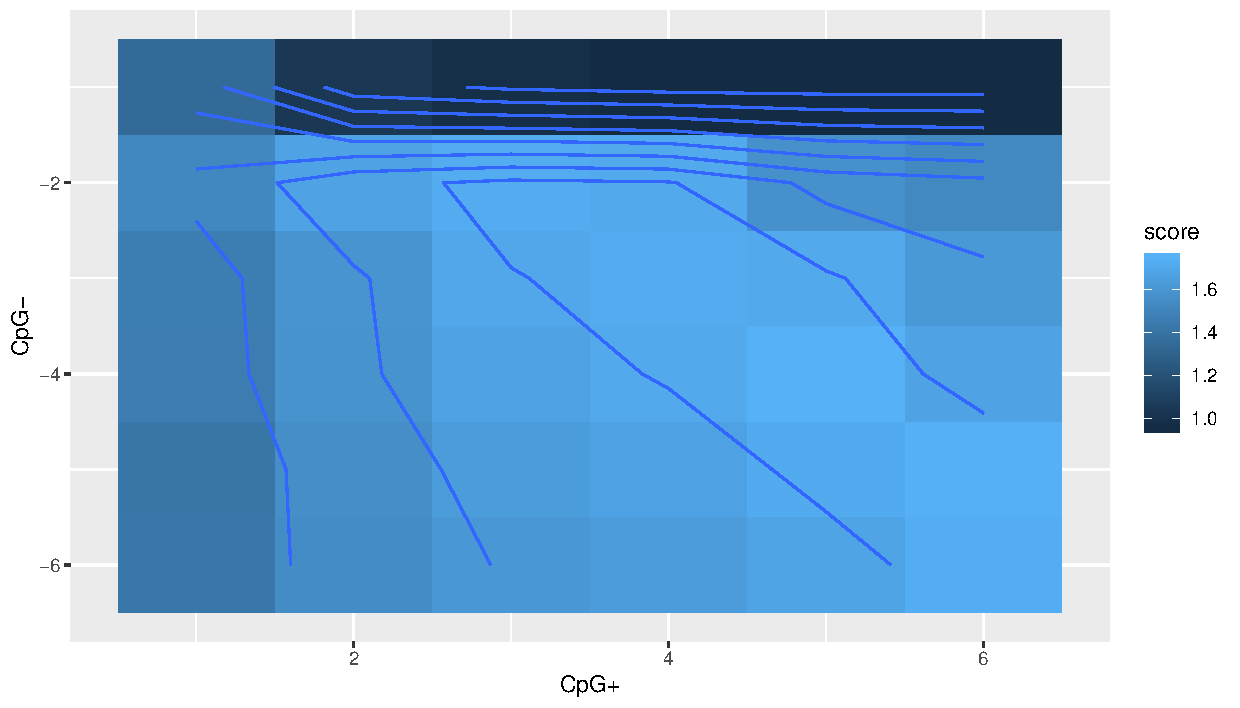
\includegraphics[width=0.59\textwidth]{fig/visual.pdf}
\end{center}
\caption{\textbf{Répartition des effectifs dans les classes de variables qualitatives.} 
%Abbréviation des variables (oui / non par défaut) : STA-Status (Vie / Mort), GENDER, RACE (Blanc / Noir / Autre), SER-Admission (Medical / Chirurgie), CAN-Cancer en cause, CRN-Maladie de rein chronique, INF-Infection probable, CPR, PRE-précédente admission (6mois), TYP-Admission/Urgence, FRA-fracture, PO2-Dioxygen (> 60 / < 60), PH (> 7.25 / < 7.25), PCO2-Dioxide de carbone (< 45 / > 45), BIC-Bicarbonate (> 18 / < 18), CRE-Creatinine(< 2.0 / > 2.0), LOC-Conscience (Stupeur / Inconscient / Coma)
}
\vspace{-20pt}
\label{fig:visual}
\end{wrapfigure}

Alors, avant la réalisation d'un possible modèle expliquant les observations, il sera néccessaire de limiter les biais introduits par ces variables. On peut donc dans un premier temps supprimer la variable `RACE`, car l'assignation des individus ne repose pas sur une mesure précise. Afin d'écarter d'autres variables qualitatives, leurs corrélations ont été évalués au moyen d'un test de $\chi^2$ par paires de variables.


\begin{table}[h]
  \begin{center}
  % latex table generated in R 3.4.4 by xtable 1.8-3 package
% Tue Oct 29 18:56:15 2019
\begingroup\tiny
\begin{tabular}{rlllllllllllllll}
  \hline
 & GENDER & SER & CAN & CRN & INF & CPR & PRE & TYP & FRA & PO2 & PH & PCO & BIC & CRE & LOC \\ 
  \hline
GENDER & NA & NA & NA & NA & NA & NA & NA & NA & NA & NA & NA & NA & NA & NA & NA \\ 
  SER & - & NA & 0.0035 & 0.05 & 0.003 & 0.002 & NA & 5e-04 & 0.0145 & 0.003 & 0.001 & 0.027 & 5e-04 & 0.044 & NA \\ 
  CAN & - & - & NA & NA & NA & NA & NA & 5e-04 & NA & NA & NA & NA & NA & NA & NA \\ 
  CRN & - & - & - & NA & NA & 0.0235 & NA & NA & NA & NA & 0.023 & NA & 0.0355 & 0.002 & 0.034 \\ 
  INF & - & - & - & - & NA & 0.041 & 0.0155 & 0.0225 & NA & 0.007 & 0.01 & 0.034 & 0.0135 & NA & NA \\ 
  CPR & - & - & - & - & - & NA & NA & 0.0405 & NA & NA & NA & NA & NA & NA & 0.001 \\ 
  PRE & - & - & - & - & - & - & NA & NA & NA & NA & NA & NA & NA & NA & NA \\ 
  TYP & - & - & - & - & - & - & - & NA & NA & NA & NA & NA & 0.035 & NA & NA \\ 
  FRA & - & - & - & - & - & - & - & - & NA & NA & NA & NA & NA & NA & NA \\ 
  PO2 & - & - & - & - & - & - & - & - & - & NA & 0.002 & 5e-04 & 0.026 & NA & NA \\ 
  PH & - & - & - & - & - & - & - & - & - & - & NA & 5e-04 & 0.002 & NA & NA \\ 
  PCO & - & - & - & - & - & - & - & - & - & - & - & NA & NA & NA & NA \\ 
  BIC & - & - & - & - & - & - & - & - & - & - & - & - & NA & 0.003 & NA \\ 
  CRE & - & - & - & - & - & - & - & - & - & - & - & - & - & NA & NA \\ 
  LOC & - & - & - & - & - & - & - & - & - & - & - & - & - & - & NA \\ 
   \hline
\end{tabular}
\endgroup

  \end{center}
  \caption{\textbf{P-valeurs des tests de $\chi^2$ par paires de variables qualitatives sur 70\% du jeu de donnée.} Les cases avec `NA` indiquent des valeurs > 0.05.}
  \label{table:quali_cor}
\end{table}     

Il apparaît qu'effectuer ces tests de $\chi^2$ sur un plus petit jeu de données entraîne une dimition du nombre de corrélations. Pour les corrélations restantes après un échantillonnage, la variable `SER` est corrélée au plus d'autres variables. De même `PCO` est corrélée à 4 autres variables (Table \ref{table:quali_cor}). Il existe d'autres variables corrélées, mais il semble préférable de limiter le nombre de variables explicatives et de favoriser le choix de variables corrélées à plusieurs autres et dont les classes sont les moins déséquilibrées possibles (Figure \ref{fig:visual}). Parmis les variables qualitatives seront donc conservés : `SER`, `INF`, `PRE`, `TYP` et `PCO`.


Afin de limiter le nombre de variables, une analyse de corrélations entre les variables quantitatives est aussi réalisé. Les deux variables `HRA` (Rythme cardiaque) et `SYS` (Pression systolique) ne présentent pas des répartitions suivant une loi normale, avec une P-valeur au test de Shapiro de respectivement 3.1 et 3.1, permettant de rejeter H0. Un test de corrélation de Kendall ne permet pas de souligner une corrélation entre les deux variables, avec une p-valeur de 3.1.


À vue des coïncidences entre variables, les modèles considerés partiront de sept variables pour expliquer la variable binomiale `STA`, qui indique la survie ou non du patient à l'issue de son séjour en service de soins intensifs. Ces variables sont : le sexe du patient (`GENDER`), son âge (`AGE`), la raison de son admission -médicale / chirurgicale- (`SER`), la présence d'une infection lors de l'admission (`INF`), une précédente admission dans les derniers 6 mois (`PRE`), la nature de l'admission -prévue / urgence- (`TYP`) et la pression en dioxide de carbone dans le sang à l'admission (`PCO`). Le choix du meilleur modèle sera d'abord effectué sur un sample du 70\% du jeu de données, ensuite généralisés à la totalité des données. 

\subsection*{Modélisation}

La selection de modèle avec plusieurs variables se fait par selection stepwise, au moyen de la fonction \verb|stepAIC| du package \verb|MASS|. Cette analyse est portée sur un jeu de donnée échantillonné ainsi que sur l'ensemble du jeu de données. Dans les deux cas, les variables choisies comme celles les plus discriminantes pour la survie sont l'âge de l'individu, la pression systolique lors de l'admission et le type d'admission. 



Des analyses successifs du test de Wald et du test de rapport de vraisemblance confirment que les variables 'AGE', 'SYS' ou 'TYP' séparémment ne servent pas à expliquer assez de déviation des résidus: le modèle avec les trois variables ensemble est significativement meilleur que les trois modèles n'incluant que l'une d'elles à la fois, avec des moindres valeurs de déviation des résidus pour toutes les trois. 

\begin{table}[h]
  \begin{center}
  % latex table generated in R 3.4.4 by xtable 1.8-3 package
% Tue Oct 29 18:56:16 2019
\begin{tabular}{rrrr}
  \hline
 & AGE & SYS & TYP \\ 
  \hline
Dév. modèle 1 variables & 133.19 & 132.73 & 123.11 \\ 
  Dév. modèle 3 variables & 104.31 & 104.31 & 104.31 \\ 
   \hline
\end{tabular}

  \end{center}
  \caption{Déviation des résidus selon les modèles utilisés pour chacune des variables dans le cas du jeu de donnée échantillonné.}
  \label{table:result1}
\end{table}

De cette manière, on peut conclure que le modèle doit intégrer ces trois variables pour décrire la plupart des données. Le meilleur modèle à aborder est donc : \verb|STA ~ TYP + AGE * SYS |.  


\subsection*{Validation du modèle}
Le test de Hosmer \& Lemeshow soutient l'hypothèse que le modèle est compatible avec les données du sample 70\%, même si la p-valeur est proche de 0.05 (3.1). La distance de Cook ne montre pas de points influents, ce qui nous fait accepter les observations du dataset. 

\begin{figure}
\vspace{-20pt}
\begin{center}
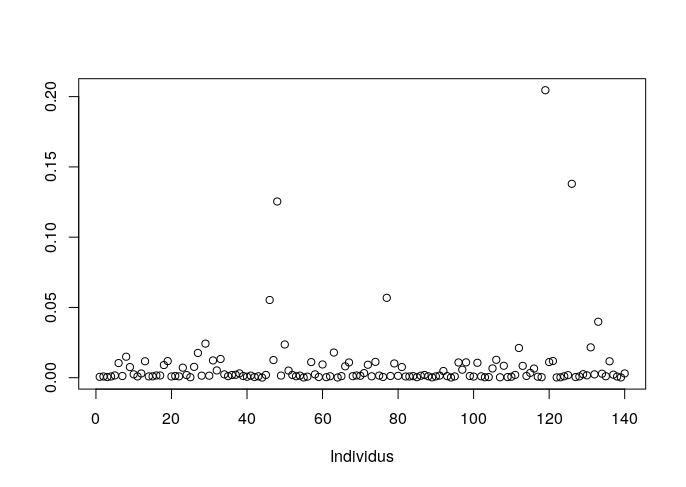
\includegraphics{fig/Rplot.png}
\caption{Répartitions des distances de Cook pour le jeu de données échantillonné.}
  \label{table:cooks}
\end{center}
\end{figure}


\subsection*{Performance du modèle}
La surface en dessous de la courbe ROC (dîte valeur AUC) est de 3.1. Ce modèle ne semble pas être très performant, vu la grande surface en dessous de la courbe et la valeur de sensibilité de 3.1, laquelle fait preuve du grand nombre de faux positifs. Les valeurs de AUC et de sensibilité s'améliorent relativement pour la totalité du jeu de données, avec un AUC de 3.1 et une sensibilité de 3.1.  


Le choix du modèle était bien basé vu que, pour le sample 70\%, les modèles contenant les trois variables 'AGE', 'TYP' et 'SYS' servaient à expliquer plus de variabilité des données que ceux ne contenant qu'une d'elles. C'est aussi le cas si l'on teste ces mêmes conclusions sur le jeu de données complet. \

\begin{table}[h]
  \begin{center}
  % latex table generated in R 3.4.4 by xtable 1.8-3 package
% Tue Oct 29 18:56:16 2019
\begin{tabular}{rrrr}
  \hline
 & AGE & SYS & TYP \\ 
  \hline
Dév. modèle 1 variables & 192.31 & 191.34 & 185.05 \\ 
  Dév. modèle 3 variables & 167.82 & 167.82 & 167.82 \\ 
   \hline
\end{tabular}

  \end{center}
  \caption{Déviation des résidus selon les modèles utilisés pour chacune des variables dans le cas du jeu de donnée entier.}
  \label{table:result2}
\end{table} 

C'est vrai que l'approche stepwise pour le dataset complet propose des effets croisés entre l'âge et la pression systolique comme explication d'une part de la variabilité des données. Une fois ajouté le terme des effets croisés, les valeurs de AUC et de sensibilité s'améliorent relativement avec un AUC de 3.1 et une sensibilité de 3.1.


\subsection*{Conclusion}

L'analyse permet donc de faire ressortir des variables intéressantes sur la survie des patients aux services de soins intensifs. Cependant cette analyse n'est pas exhaustive et la faible différence de modèles avant et après échantillonnage questionne sur la qualité du jeu de donnée, et sa taille réduite. Il faut également remarquer que le modèle proposé est réduit à une régression logistique et que d'autres interractions peuvent avoir leurs importances dans la survie du patient.

%\SweaveInput{child_test.Rnw}

%\end{multicols}
\fi

% %%%%%%%%%%%%%%%%%%%%%%%%%%%%%%%%%%%%%%%%%%%%%%%%%%%%%%%%%%%%%%%%%%%%%%
% % Références
% %%%%%%%%%%%%%%%%%%%%%%%%%%%%%%%%%%%%%%%%%%%%%%%%%%%%%%%%%%%%%%%%%%%%%%
% %\newpage
% \begin{multicols}{2}
% 
% \subsection*{Bibliographie}
% \bibliographystyle{authordate1}
% \bibliography{../../../../Mendeley/Markov}
% 
% \end{multicols}

%%%%%%%%%%%%%%%%%%%%%%%%%%%%%%%%%%%%%%%%%%%%%%%%%%%%%%%%%%%%%%%%%%%%%%
% Annexes
%%%%%%%%%%%%%%%%%%%%%%%%%%%%%%%%%%%%%%%%%%%%%%%%%%%%%%%%%%%%%%%%%%%%%%
% \newpage
% \begin{landscape}
% 
% \begin{annexe}
% 	\centering
% \rowcolors{2}{white}{gray!25}
% \resizebox{27cm}{!}{%
% 	\begin{tabular}{cccccccccccc}
% 	\toprule
% Species &Locality &Code &Morph &Collector &Date &Longitude &Latitude &Altitude&Reads raw &Reads trimmed &Voucher \\
% 	\midrule
% P. apennina* &Sella del Marmagna, Italy &AMB &Short-styled &F. Boucher/L. Gallien &30/05/14 & 10.00575 & 44.3978 &1610&6885928&6486849&Photo \\
% P. apennina &Monte Marmagna, Italy &AML &Long-styled &F. Boucher/L. Gallien &30/05/14 & 9.99731 & 44.39672 &1825&1856867&1663377&Photo \\
% P. apennina &Monte Orsaro, Italy &AOL &Long-styled &F. Boucher/L. Gallien &30/05/14 & 9.99666 & 44.39883 &1818&3494081&3230296&Photo \\
% P. cottia &Below locus classicus, Italy &CS1 & NA &F. Boucher &23/07/14 & 7.0716 & 44.9271 &1159&5127416&4814386&Photo \\
% 	\bottomrule
% 	\end{tabular}}
% 	\caption{\textbf{Individus séquencés pour cette étude}. D'après les informations de \citet{Boucher2016a}.}
% 	\label{table_ind}
% \end{annexe}
% \end{landscape}

\end{document}
%%%%%%%%%%%%%%%%%%%%%%%%%%%%%%%%%%%%%%%%%%%%%%%%%%%%%%%%%%%%%%%%%%%%%%
% Figures et raccoucis!
%%%%%%%%%%%%%%%%%%%%%%%%%%%%%%%%%%%%%%%%%%%%%%%%%%%%%%%%%%%%%%%%%%%%%%
%{\let\thefootnote\relax\footnote{{ \textit{Primula hirsuta},  Crédit photo : Florian Boucher}}}


% \input{fig/tset.tex}
% Je teste de mettre un tableau et ça tourne mal \ref{tset}.

% # 1. id : identifiant du sujet. Chaque observation a un identifiant unique soit une observation
% # par individu.
% # 2. STA : Vital Status (0=Lived / 1=Died)
% # 3. AGE : Age (Years)
% # 4. GENDER : Gender (0 = Male / 1 = Femal)
% # 5. RACE : Race (1 = White / 2 = Black / 3 = Other)
% # 6. SER : Service at ICU Admission (0 = Medical / 1 = Surgical)
% # 7. CAN : Cancer Part of Present Problem (0 = No / 1 = Yes)
% # 8. CRN : History of chronic renal failure (0 = No / 1= Yes)
% # 9. INF : Infection Probable at ICU Admission (0 = No / 1= Yes)
% # 10. CPR : CPR Prior to ICU Admission (0 = No / 1= Yes)
% # 11. SYS : Systolic Blood Pressure at ICU Admission mm Hg
% # 12. HRA : Heart Rate at ICU Admission Beats/min
% # 13. PRE : Previous Admission to an ICU within 6 Months (0 = No / 1= Yes)
% # 14. TYP : Type of Admission (0 = Elective / 1 = Emergency)
% # 15. FRA : Long Bone, Multiple, Neck, Single Area, or Hip Fracture (0 = No / 1= Yes)
% # 16. PO2 : from Initial Blood Gases (0 = > 60 / 1 = < 60)
% # 17. PH : from Initial Blood Gases (0 => 7.25 / 1 =< 7.25)
% # 18. PCO2 from initial Blood Gases (0 = < 45 / 1 = > 45)
% # 19. BIC : Bicarbonate from InitialBlood Gases (0 = > 18 / 1 = < 18)
% # 20. CRE : Creatinine from Initial Blood Gases (0 = < 2.0 / 1 = > 2.0)
% # 21. LOC : Level of Consciousness at ICU Admission (O = No Coma or Stupor / 1 = Deep / 2 = Coma)


%%%%%%%%%%%%%%%%%%%%%%%%%% notes pour tableau
% \begin{table}[h]
% \caption{A table with notes in the end}
%   \begin{center}
%      \begin{threeparttable}
%        % INPUT YOUR TEX HERE :
%        % latex table generated in R 3.4.4 by xtable 1.8-3 package
% Tue Oct 29 18:56:15 2019
\begingroup\tiny
\begin{tabular}{rlllllllllllllll}
  \hline
 & GENDER & SER & CAN & CRN & INF & CPR & PRE & TYP & FRA & PO2 & PH & PCO & BIC & CRE & LOC \\ 
  \hline
GENDER & NA & NA & NA & NA & NA & NA & NA & NA & NA & NA & NA & NA & NA & NA & NA \\ 
  SER & - & NA & 0.0035 & 0.05 & 0.003 & 0.002 & NA & 5e-04 & 0.0145 & 0.003 & 0.001 & 0.027 & 5e-04 & 0.044 & NA \\ 
  CAN & - & - & NA & NA & NA & NA & NA & 5e-04 & NA & NA & NA & NA & NA & NA & NA \\ 
  CRN & - & - & - & NA & NA & 0.0235 & NA & NA & NA & NA & 0.023 & NA & 0.0355 & 0.002 & 0.034 \\ 
  INF & - & - & - & - & NA & 0.041 & 0.0155 & 0.0225 & NA & 0.007 & 0.01 & 0.034 & 0.0135 & NA & NA \\ 
  CPR & - & - & - & - & - & NA & NA & 0.0405 & NA & NA & NA & NA & NA & NA & 0.001 \\ 
  PRE & - & - & - & - & - & - & NA & NA & NA & NA & NA & NA & NA & NA & NA \\ 
  TYP & - & - & - & - & - & - & - & NA & NA & NA & NA & NA & 0.035 & NA & NA \\ 
  FRA & - & - & - & - & - & - & - & - & NA & NA & NA & NA & NA & NA & NA \\ 
  PO2 & - & - & - & - & - & - & - & - & - & NA & 0.002 & 5e-04 & 0.026 & NA & NA \\ 
  PH & - & - & - & - & - & - & - & - & - & - & NA & 5e-04 & 0.002 & NA & NA \\ 
  PCO & - & - & - & - & - & - & - & - & - & - & - & NA & NA & NA & NA \\ 
  BIC & - & - & - & - & - & - & - & - & - & - & - & - & NA & 0.003 & NA \\ 
  CRE & - & - & - & - & - & - & - & - & - & - & - & - & - & NA & NA \\ 
  LOC & - & - & - & - & - & - & - & - & - & - & - & - & - & - & NA \\ 
   \hline
\end{tabular}
\endgroup

%      \begin{tablenotes}
%        \item[1] aaaa; \item[2] bbbb
%      \end{tablenotes}
%     \end{threeparttable}
%    \end{center}
%  \label{table:tablewithnotes}
%  \end{table}   
